\chapter{Results}
\label{Chapter-Results}
This chapter has three aims. First, to quantify the performance of the FPGA implementation of the ANN and analyze its resource consumption and timing. Second, to compare it will equivalent implementations on other technologies. Final and main goal, to study the interaction and discover any possible synergies or conflicts between the two technologies under focus, namely FL and FPGA. % aims

It should be noted that the following timings were produced through actual runs in a real FPGA. In the following subsections it is explained in detail how they were generated and what they actually mean.

\subsection*{Performance Metrics}

\subsubsection{Latency}
Latency, is the required time to complete a single task. In this work, latency can be the time taken to process a single image, a batch of images, a dataset of images, etc. % what is latency

\subsubsection{Throughput}
Throughput is generally referred to as the quantity of tasks completed in a given amount of time. The rate at which something is processed increases with throughput. Throughput in this work is referred to as the number of images processed per second. % what is throughput
\begin{equation}
	Throughput \coloneqq \frac{Images}{Time (sec)}
	\label{eqn: Throughput definition}
\end{equation}

\section{FPGA Implementation Analysis}

\subsection{Resource Utilization Analysis}
Although consisting of only $\sim$105000 variables and 6 layers, the implemented ANN consume a lot of resources. It has full floating point accuracy, back-propagation is employed for training, and the SGD optimization algorithm makes use of momenta. When applied in programmable logic, all of these techniques are known to significantly increase resource usage. Table \ref{table: Resource Utilization} depicts the utilization of the major resources after synthesis, place and route; according to the Vitis IDE. % resource consumpion
\begin{table}[H]
    \center
    \begin{tabular}
        { | l | r | r | r | }
        \hline
        Resource & Utilization & Available & Utilization \%\\
        \hline
        LUT      & 161274 & 274080 & 58.84\\
        LUTRAM   &  14270 & 144000 &  9.91\\
        FF       & 260050 & 548160 & 47.44\\
        BRAM     &    573 &    912 & 62.83\\
        DSP      &    854 &   2520 & 33.89\\
        \hline
    \end{tabular}
    \caption[Resource Utilization]{Post place \& route resource utilization.}
    \label{table: Resource Utilization}
\end{table}
The highest use rate is observed on the BRAM. It is intrinsically tied to the size of the ANN due to three key factors. Firstly, to enable the quickest access to the ANN's variables, they are stored in on-chip memory. Furthermore, the back-propagation algorithm demands the temporary storage of all data that bypass hardware functions. Lastly, between each batch update, the SGD algorithms' momenta must be saved. %BRAM comment

The utilization of the rest of the PL is affected mostly on the desired accuracy and the applied parallelism. Using single precision floating points is more resource demanding than using half precision and less than using double precision. Although it appears there is space to improve parallelism, the benefits diminish the more that this is done. Most crucially, timing-based constraints rather than resource-based constraints are the biggest barriers to it. %the rest comment

\subsection{Timing Analysis}
A thorough analysis of the implementation's timings is required to to assess its performance, identify delays and limitations, as well as enable future improvements. This section provides a breakdown of the relevant latencies. The following formulas and results have been confirmed by experiments on the ZCU102. % why analize timing

\subsubsection{Overall Latency}
From the point of view of the host program, the overall latency of training can be broken down as follows; writing the variables in global memory, calling the accelerator, waiting for the accelerator to return, and finally read the produced variables from the global memory. % host latency
\begin{equation}
	Host_{latency} = GMEM_{write} + Accel_{call} + Accel_{wait} + GMEM_{read}
	\label{eqn: host program, training latency}
\end{equation}
Important to note, all parts involve system calls to the operating system, which can introduce a small variance in their latency. Additionally, in the case of the FL client with the map API, the latency of accessing the global memory is hidden under the FL operation, as the socket reads and writes there directly. % comments

\subsubsection{Accelerator's Latency}
Accountable for the majority of the overall latency is waiting for the accelerator to finish running. As observed in figure \ref{fig: top function}, its operation consists of initializing its on-chip local memory, calculating the gradients, updating the variables, and finally writing the final variables to the global memory. % parts of accel latency

The first and the last segments are executed only once and they are independent of any variable such as the size of the dataset used for training. In contrast, the two dataflow regions, generating the gradients and updating the trainable variables, are repeated multiple times depending on the number of training epochs and the number of batches in the dataset. in more detail: % what is repeated
\begin{equation}
    Accel_{latency} = I + e \cdot \frac{d}{b} [ G(b) + U ] + S
    \label{eqn: Accel, training latency}
\end{equation}
Where:
\begin{conditions}
    I & initialize inputs\\
    e & training epochs\\
    d & dataset size\\
    b & batch size\\
    G & calculate the gradients\\
    U & update trainable variables\\
    S & Save final variables\\
\end{conditions}
Calculating the gradients is done using the long and complex pipeline depicted in figure \ref{fig: Gradients Calculation Pipeline Block Diagram}. It has significant wind-up and wind-down latencies and its total run-time is dependent on the batch size. % gradients calculation analysis
\begin{equation}
    G(b) = G_{up} + b \cdot E + G_{down}
    \label{eqn: Gradients pipeline, training latency}
\end{equation}%
Where:
\begin{conditions}
    G_{up} & latency to wind-up the pipeline\\
    G_{down} & latency to wind-down the pipeline\\
    E & latency added by one example\\
\end{conditions}
Thus, the latency of the accelerator can better be described as:
\begin{equation}
    Accel_{latency} = I + S + e \cdot d [ E + \frac{ G_{up} + G_{down} + U }{b} ] % 24613 + 60000 [ 33320 + ( 35310 + 25121 )/b ]
    \label{eqn: Accel, training latency, complete}
\end{equation}
$U$, as described in section \ref{sec:Updating_Variables}, is completely elastic and the main target when optimizing for small batches.

Through analyzing the Vitis reports, exact numbers can be assigned on each constant. For a single pass through the whole dataset $( e=1, d=60000 )$ and a clock speed of $4.08 ns (\sim245MHz)$, the equation transforms to: % function with numbers
\begin{equation}
    Accel_{latency} = 8.157 + \frac{ 14.794 }{b} (sec) % 1999224613 + 3625860000/b 
    \label{eqn: accel, training latency in ms}
\end{equation}
\subsubsection{Constrains}
\label{Constrains}
According to equation \ref{eqn: Accel, training latency, complete}, the latency introduced by each example (E) is the most important constant. Accountable for that is the dataflow region shown in figure \ref{fig: Gradients Calculation Pipeline Block Diagram}, thus received most of the optimization attention. Better performance is restricted mostly by a single issue caused by the HLS tool, affecting clock speed and the total operating clock cycles. % importance of E and issues

The slowest function of a dataflow region determines its overall latency. In this case, it is the \textit{sum filters} in the back-propagation of the second convolutional layer. Per example, it has 14$\times$14 inputs with 32 input and 16 output channels. The outputs are independent from each other and are calculated in parallel. Thus, 16 accumulators that reset every 32 cycles are needed. % where is problem

Unfortunately, in the latest versions of the Vitis HLS, the tool can not deduce that the \textit{facc} operator is the optimal choice if its accuracy has not been set to low. Instead, when normal accuracy is requested, it implements the slower \textit{fadd} operator, which forces an II of 5 cycles and a clock speed of 245MHz. As a result, the latency of a single example is at least 31360 cycles. % what is the problem and what it affects

The next slowest functions are the \textit{create windows} hardware functions in the convolutional and maxpool layers (layers 0 to 3). While they are simple data transformation, the HLS tool encounters some difficulty in implementing them efficiently, as they are composed mostly of control logic. Still, it is able to synthesize them with a clock of over 300 MHz.% Furthermore, it is unable to always synthesize them with a free running pipeline, requiring deeper input and output streams to guarantee robustness against random stalls. % next slowest

Both cases are byproducts of using HLS tools. If just the \textit{facc} bug is avoided, the clock can be immediately increased by 55MHz. Without trying to improve the II of the function, the latency equation transforms to: % Creating these two function using RTL, would greatly improve the overall performance.  % change with facc
\begin{equation}
    Accel_{latency} = 6.664 + \frac{ 12.086 }{b} (sec) % 1999224613 + 3625860000/b
    \label{eqn: Accelerator with facc, training latency in ms}
\end{equation}
Visualizing the equations \ref{eqn: accel, training latency in ms} \& \ref{eqn: Accelerator with facc, training latency in ms} in the diagram \ref{fig: accel latency}, shows that their second part is insignificant for batches of over 100 images. In contrast, the first part is unavoidable and sets a base latency regardless of the batch size. % visualize
\begin{figure}[H]
    \center
    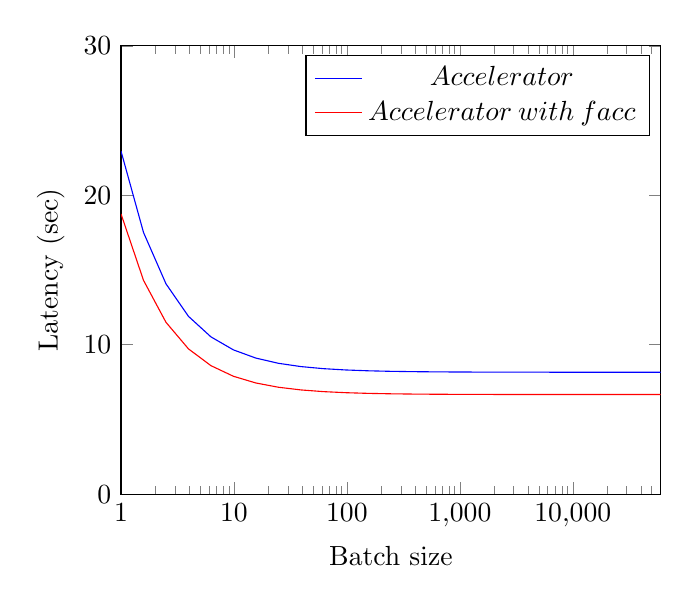
\begin{tikzpicture}
        \begin{axis}[
            xmode = log,
            log ticks with fixed point,
            ymin = 0,
            ymax = 30,
            xmin = 1,
            xmax = 60000,
            ylabel = Latency (sec),
            xlabel = Batch size
        ]
            \addplot[ domain = 1:60000, color = blue ] { 8.156836421 + 14.793508800 / x };
            \addplot[ domain = 1:60000, color = red ] { 6.664082036 + 12.086199879 / x };
            \addlegendentry{$Accelerator$}
            \addlegendentry{$Accelerator\:with\:facc$}
        \end{axis}
    \end{tikzpicture}
    \caption[Accelerator's latency per batch size]{Latency with and without the facc module.}
    \label{fig: accel latency}
\end{figure}

\subsection{Power Consumption Analysis}
The average power consumption of the design can be reliably estimated by the Xilinx tools. This report was generated post-implementation and is shown in figure \ref{fig: power}. A breakdown of the consumption per PL element can be seen.

\begin{figure}[H]
    \centering
        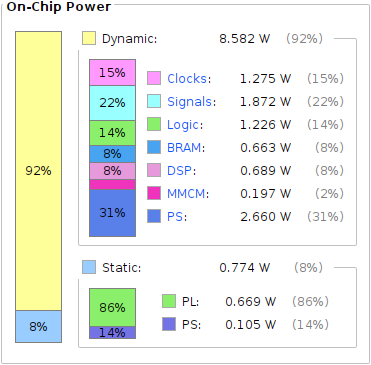
\includegraphics{Images/power.png}
        \decoRule
        \caption[Power Estimation]{Post-implementation power estimation of the accelerator.}
        \label{fig: power}
\end{figure}

The average consumption is stated as 9.356 W, with the PL accountable for the majority of it. This is to be expected, as the PS part of the accelerator mostly does nothing while waiting for the PL part to finish. In practice, most of the PS consumption is sourced from the of-chip memory used.

\section{Comparison with Other Technologies}
To form an opinion on the efficiency of the FPGA implementation, a proper comparison is required. Thus, the ANN is also trained on CPU and GPU using TensorFlow. As metrics, the latency of a training epoch and the overall throughput are used.

\subsection{Specification of Compared Platforms}
\subsubsection{Intel Core i7-9750H}
Released in mid 2019, the i7-9750H is a high end CPU for laptops. Based on the Coffee Lake architecture and manufactured with the 14nm++ process, it provides a wide array of technologies such as Hyper-Treading and SIMD Instruction Set Extensions, making it suitable for training the ANN under consideration. Furthermore, TensorFlow has been compiled with AVX instructions enabled. % CPU
\begin{table}[H]
    \center
    \begin{tabular}
        { l | l }
        Core / Threads & 6 / 12\\
        Clock Frequency & 2.6 - 4.5 GHz\\
        Cache & 12 MB Intel Smart Cache\\
        Supplied Memory & 16GB DDR4-2666\\
        Max Memory Bandwidth & 41.8 GB/s $\times$ 2 channels\\
        Instruction Set Extensions & SSE4.1, SSE4.2, AVX2\\
        Average Power Consumption & 45 W\\
    \end{tabular}
    \caption[i7-9750H specifications]{i7-9750H specifications \cite{i7-9750H}.}
    \label{table: i7-9750H}
\end{table}

\subsubsection{Nvidia GTX 1660 Ti}
While released in early 2019 as mobile platform (laptops, tablets, etc.) GPU, is more than capable for training ANNs like the one under investigation. Its relevant specifications are shown on the following table. % GPU
\begin{table}[H]
    \center
    \begin{tabular}
        { l | l }
        CUDA cores & 1536\\
        Clock Speed & 1500 - 1770 MHz\\
        Memory Configuration & 6GB GDDR6, 1500 MHz\\
        Memory Interface & 192-bit\\
        Memory Bandwidth & 288 GB/s\\
        Single Precision Compute Power & 5437.44 GFLOPS\\
        Compute Capability & 7.5\\
        Average Power Consumption & 120 W\\
    \end{tabular}
    \caption[GTX 1660 Ti specifications]{GTX 1660 Ti specifications \cite{GTX1660Ti}.}
    \label{table: GTX1660Ti}
\end{table}

\subsection{Latency Comparison}

\begin{figure}[H]
    \center
    \begin{tikzpicture}
        \begin{axis}[
            xmode = log,
            log ticks with fixed point,
            ymin = 0,
            ymax = 110,
            xmin = 1,
            xmax = 60000,
            ylabel = Latency (sec),
            xlabel = Batch size,
            scale = 1.25,
            no markers
        ]
            \addplot[ domain = 1:60000 , color = blue ] { 8.166836421 + 14.793508800 / x };
            \addlegendentry {$FPGA$}
            
            \addplot+ [ forget plot , name path=upper_gpu , draw=none ] table[ smooth , tension=.8 , x=batch_size , y=latency_max ] {data/gpu_latency_per_batch_size.dat};
            \addplot [ name path=lower_gpu , color=red ] table[ smooth , tension=.8 , x=batch_size , y=latency_min ] {data/gpu_latency_per_batch_size.dat};
            \addplot+ [ forget plot , fill=red!25 ] fill between[ of=upper_gpu and lower_gpu ];
            \addlegendentry {$GPU$}

            \addplot+ [ name path=upper_cpu , color=green ] table[ smooth , tension=.8 , x=batch_size , y expr = ( \thisrow{latency_max} + \thisrow{latency_min} ) / 2 ] {data/cpu_latency_per_batch_size.dat};
            \addlegendentry {$CPU$}
        
        \end{axis}
    \end{tikzpicture}
    \caption[FPGA, GPU, CPU latency comparison]{Latency of training for a single epoch on FPGA, GPU and CPU}
    \label{fig: FPGA CPU GPU latency}
\end{figure}

Due to the CPU's fluctuating clock speed and caching architecture, training latency has a slight variance. This effect is considerably more pronounced on the GPU, as it also copy the training dataset and the ANN's variables to its dedicated memory, during the first epoch. % variance CPU, GPU

On the FPGA, however, training latency is practically deterministic. The only variance that it encounters, is produced by the system calls and is less than 10 ms. Such effects should be noted as this work also considers on-edge devices, where the training algorithm may not have complete control over them and their environment is not always in an ideal state. % variance GPU

Performance wise, according to figure \ref{fig: FPGA CPU GPU latency}, the FPGA implementation outperforms in training with small batches, but is overtaken by the GPU when their size is larger than or equal to 15 examples. Training on CPU is consistently slower than the other technologies.

It should be noted that the GPU is unable to perform non-Stochastic Gradient Descent, where the whole dataset is concatenated in a batch. TensorFlow can not obtain enough GPU dedicated memory and crashes. Due to non-determinism in memory management, this can also occur for SGD with batches of more than 15000 samples. In on-edge devices, such effects are expected to become more noticeable, due to the FL algorithm's limited control.

\subsection{Throughput Comparison}
\begin{figure}[H]
    \center
    \begin{tikzpicture}
        \begin{axis}[
            ymode = log,
            xmode = log,
            % log ticks with fixed point,
            ymin = 100,
            ymax = 100000,
            xmin = 1,
            xmax = 60000,
            ylabel = Throughput (Images/sec),
            xlabel = Batch size,
            scale = 1.25,
            no markers,
            legend pos = south east
        ]
            \addplot[ domain = 1:60000 , color = blue ] { 60000 / ( 8.166836421 + 14.793508800 / x ) };
            \addlegendentry {$FPGA$}
            
            \addplot+ [ color=black ] table[ smooth , tension=.8 , x=batch_size , y expr={ 60000 / \thisrow{latency_max} } ] {data/gpu_latency_per_batch_size.dat};
            \addlegendentry {$GPU$, worst}
            
            \addplot+ [ color=red ] table[ smooth , tension=.8 , x=batch_size , y expr={ 60000 / \thisrow{latency_min} } ] {data/gpu_latency_per_batch_size.dat};
            \addlegendentry {$GPU$, best}

            \addplot+ [ color=green ] table[ smooth , tension=.8 ,
                x=batch_size ,
                y expr={ 60000 / ( ( \thisrow{latency_max} + \thisrow{latency_min} ) / 2 ) } ] 
                {data/cpu_latency_per_batch_size.dat};
            \addlegendentry {$CPU$}
        
        \end{axis}
    \end{tikzpicture}
    \caption[FPGA, GPU, CPU throughput comparison]{Throughput of FPGA, GPU and CPU implementations}
    \label{fig: FPGA CPU GPU throughput}
\end{figure}
Similar observations can be made by comparing the throughput of the implementations in figure \ref{fig: FPGA CPU GPU throughput}. Although the FPGA starts from more than 2600 images per second, its performance plateaus at around 7500. In contrast, the GPU can only achieve ~600 images per second with single image batches, but reaches a maximum throughput of 50000 when using huge batches.

\subsection{Power Consumption Comparison}
Table \ref{table: power} presents the power consumption of the three implementation. An actual system with the CPU or GPU implementation, would require other components to operate, e.g. a motherboard. In contrast, the FPGA-based implementation is aimed for the ZCU102, which is an SoC, and requires no other components. This is a gross comparison, and aims to give a general idea of their differences.
\begin{table}[H]
    \center
    \begin{tabular}
        { | c | c | c | }
        \hline
        CPU & GPU & FPGA\\
        \hline
        53 W & 120 W & 9.356 W\\ 
        \hline
    \end{tabular}
    \caption[Power Consumption]{Power consumption of the three implementations.}
    \label{table: power}
\end{table}
Although the CPU's average power usage is listed as 45 W, during actual runs it rises to 53 W due to clock frequency boosting. The FPGA consumes \(5.67\times\) less power than the CPU and \(12.83\times\) less power than the GPU.


\section{FL \& FPGA Interaction Analysis}
\subsection{Methodology}
The main objective of this study, to investigate how FL and FPGAs interact, is explored in this section. Merely comparing the throughput of the implementations is inadequate since, as demonstrated in chapter \ref{Chapter-Robustness-Analysis}, the number of global epochs depends on a multitude of factors. The batch size is the element that has the greatest impact on both FL and local training. As a result, it is the central factor of the experiments. % objective, why focus on batch size

Another factor that has a significant impact is the LR degradation. Through experimentation, the most effective tactic was determined to be decreasing a client's LR for each epoch it participates. Depending on the batch size, different rates of that decrease were the most efficient. To ensure fairness on the following experiments, they were repeated with various LR decay constants. In this section, the best results for each are presented. % LR decay

Having access to a single FPGA and a single GPU, makes running the algorithm in real time impossible, as it requires several devices. Instead, all processes, server and clients, run on the CPU to discover the number of required global epochs to reach a target accuracy, and then their training latency is replaced with that of the desired device. As all clients operate in parallel, the training latency is not depended on how many are used. % forced to simulate

The communication delay between server and clients is handled similarly. It is determined by multiplying the size of the messages with an expected communication speed. Generally, servers have high speed connections, up to 1 Gbps upload and download. In contrast, the connection speed of on-edge devices is multiple order of magnitude slower, and the deciding factor of the overall communication latency. % communication delay

Additional latencies, caused by synchronization or the computational part on the server, amount to just a few milliseconds per epoch and are consistent across all platforms. Therefore, they can conveniently be ignored. % other latencies

For the following tests, clients are configured with a download speed of 10Mbps and a upload speed of 1Mbps. Furthermore, the messages between client and server have a size of 3387808 bits. Considering that clients are operating in parallel, the latency of a Global Epoch can be described as: % GE latency
\begin{equation}
    \begin{gathered}
        GE_{latency} \simeq StoC_{latency} + LT_{latency} + CtoS_{latency}\\
                     = \frac{ StoC\_msg_{bits} }{ C\_down_{bps} } + LT_{latency} + \frac{ CtoS\_msg_{bits} }{ C\_up_{bps} }\\
                     = LT_{latency} + 3.7266 \: (sec) % 0.3388 + 3.3878
    \end{gathered}
    \label{eqn: Global Epoch Latency}
\end{equation}
Where:
\begin{conditions}
    LT & Local Training\\
    StoC & Server to Client\\
    CtoS & Client to Server\\
\end{conditions}

It should be noted that the results of the previous section can not be used in place of $LT_{latency}$. The size of the local datasets differs, depending on how the data are distributed across the clients. Thus, the latency of the local training has been re-measured for every platform. % lt remeasured

\subsection{IID} % TODO: replace X and Y with numbers
In the first experiment, the Fashion-MNIST dataset is split randomly and evenly across 10 clients. This is an IID distribution, in the sense that is used in relevant bibliography. All random factors, such as dataset distribution and client selection, have been seeded to remove their effects from the final results. % data, seeds

The model is trained with the FedAvg algorithm multiple times, once for each batch size that perfectly divides the local datasets. Out of the 10 clients, 5 of them are randomly selected to participate in each GE. The constant parameters of the experiment are listed in table \ref{table: ΙID experiment parameters}. % algorithm & parameters
\begin{table}[H]
    \center
    \begin{tabular}
        { | l | c | }
        \hline
        parameters & FedAvg\\\hline
        total clients   & 10\\\hline
        clients per GE  & 5\\\hline
        local epochs    & 1\\\hline
        initial LR      & 1e-2\\\hline
    \end{tabular}
    \caption[IID experiment parameters]{Constant parameters of the IID FL experiment.}
    \label{table: ΙID experiment parameters}
\end{table}

Each training run consists of 200 GEs or until it reaches the target accuracy of 91\%. In each GE, selected clients train their local models with their local datasets for 1 epochs. Figure \ref{fig: IID, GEs per batch size} shows the elapsed GEs to reach the target accuracy for every batch size.
\begin{figure}[H]
    \center
    \begin{tikzpicture}
        \begin{axis}[
            ybar,
            ylabel = Global Epochs,
            ymin = 0,
            ymax = 200,
            xlabel = Batch size,
            % xtick = data,
            symbolic x coords = {5,6,8,10,12,15,16,20,24,25,30,40,48,50,60,75,100,120,125,150,200},
            xtick style = {draw=none},
            scale = 1.25,
            enlarge x limits={abs=6pt},
        ]
            \addplot [ black , fill = blue!50 ] table [ x = batch_size , y = global_epochs] {data/IID_epochs.dat};
        \end{axis}
    \end{tikzpicture}
    \caption[ IID distribution, GEs per batch size ]{ GEs required to reach 91\% accuracy, when under IID distribution.}
    \label{fig: IID, GEs per batch size}
\end{figure}

Training with batch sizes of 4 or less, produces overfitted local models and renders the target accuracy unattainable. This problem could be alleviated by using a more sophisticated LR decay strategy or by distributing the dataset among more clients, but both are outside the scope of this work. % tiny batches

More interesting is the range of batch sizes from 5 to 50, where the target accuracy is reached in 30 to 60 GEs. Larger sizes increase the required number of GEs in a parabolic manner, and regardless how fast is the local training, the increase in communication most likely prohibits their use.

Figure \ref{fig: IID, total time} shows, per batch size, how much time is required to reach the target accuracy. The FPGA design is benchmarked with the best case of the GPU, where the dataset is already cached in its dedicated memory.  % final diagram what it is
\begin{figure}[H]
    \centering
    \addtolength{\leftskip} {-2cm} % increase (absolute) value if needed
    \addtolength{\rightskip}{-2cm}
    
    \begin{tikzpicture} [
        /pgfplots/every axis/.style = {
            ybar stacked ,
            bar width = 8pt,
            ymin = 0 ,
            ymax = 1000 ,
            ytick distance = 250 ,
            ylabel = Global Training time (sec) ,
            symbolic x coords = {5,6,8,10,12,15,16,20,24,25,30,40,48,50,60,75,100,120,125,150,200} ,
            enlarge x limits = 0.03 ,
            xtick = data,
            xtick style = { draw = none } ,
            xlabel = Batch size,
            width = 1.25 \textwidth ,
            height = 0.75 \textwidth ,
        }
    ]
        \begin{axis}[ bar shift = -4pt , ]
            \addplot [ black , fill = blue!75 ] 
                table [ 
                    y expr = { \thisrow{global_epochs} * ( 0.82568 + 1.47935 / \thisrow{batch_size} ) } , 
                    x = batch_size ,
                    meta expr = { \thisrow{global_epochs} * ( 0.82568 + 1.47935 / \thisrow{batch_size} ) } 
                ] {data/IID_epochs.dat};  % training cost

            \addplot [ black , fill = blue!25 ,
                point meta = y ,
                nodes near coords = \pgfmathprintnumber\pgfplotspointmeta ,
                every node near coord/.append style = {
                    font=\footnotesize ,
                    anchor = west ,
                    rotate = 90 ,
                    yshift = 4pt ,
                    /pgf/number format/.cd , precision = 0 ,
                }
            ] 
                table [ 
                    y expr = { \thisrow{global_epochs} * 3.73 } , 
                    x = batch_size , 
                    meta expr = { \thisrow{global_epochs} * 3.73 } ,
                ] {data/IID_epochs.dat}; % communication cost 
                \label{FPGA_iid} 
        \end{axis}
        
        \begin{axis}[ hide axis , bar shift = 4pt , legend pos = north west , ]
            \addplot [ forget plot , black , fill = red!75 ] 
                table [ 
                    y expr = { \thisrow{global_epochs} * ( \thisrow{gpu_lat_per_epoch} ) } , 
                    x = batch_size ,
                    meta expr = { \thisrow{global_epochs} * ( \thisrow{gpu_lat_per_epoch} ) } 
                ] {data/IID_epochs.dat};  % training cost

            \addplot [ black , fill = red!25 , 
                point meta = y ,
                nodes near coords = \pgfmathprintnumber\pgfplotspointmeta ,
                every node near coord/.append style = {
                    font=\footnotesize ,
                    anchor = west ,
                    rotate = 90 ,
                    yshift = -4pt ,
                    /pgf/number format/.cd , precision = 0
                }
            ]
                table [
                    y expr = { \thisrow{global_epochs} * 3.73 } ,
                    x = batch_size ,
                    meta expr = { \thisrow{global_epochs} * 3.73 }
                ] {data/IID_epochs.dat}; % communication cost

            \addlegendentry{GPU}
            \addlegendimage{ /pgfplots/refstyle=FPGA_iid }\addlegendentry{FPGA}
        \end{axis}
    \end{tikzpicture}
    
    \caption[ IID distribution, total time per GE ]{ Total wall-clock time to train with IID dataset distribution over 10 clients, per batch size. Darker colors = local training time, lighter colors = communication time. }
    \label{fig: IID, total time}
\end{figure}

It is apparent that communication, across all batch sizes, is the main contributor to overall latency. Considering that the dataset is split over 10 clients, 6000 examples for each one, there in not much training to be done per GE, rendering maximum throughput a secondary characteristic. Instead, the most important variables are the number of GEs and the minimum latency per GE. % com latency, what is more important

Batch sizes of 8 to 20 appear to be the sweet spot. In that range, either the FPGA has similar latency with the GPU, or it is slightly more efficient. With larger batches the GPU requires significantly less computing but, due to additional communication, the overall latency is abysmal. % best cases

\subsection{Non-IID}
Given that in real-world FL scenarios clients have different data collection and storage biases, it is exceptionally rare for the local datasets to be IID distributed. Every FL system should therefore be evaluated using non-IID data distributions. For this experiment, the FedAvg algorithm is employed, with all clients participating in every GE. % why non-IID & algorithm

The Fashion-MNIST dataset is divided among 5 clients, each of which is the exclusive owner of two labels. The first client owns all the examples with the first two labels, the second client has those with the next two labels, etc. This is a pathological non-IID distribution, arguably more unbalanced than real scenarios, but it is a great option to test the limits of the system. % data distribution

Like in the previous experiment, results are obtained with every batch size that perfectly divides the local datasets. Constant parameters are listed in table \ref{table: Non-IID experiment parameters}. Furthermore, no countermeasures for non-IID datasets, such as data rebalancing, have been utilized. % parameters
\begin{table}[H]
    \center
    \begin{tabular}
        { | l | c | }
        \hline
        parameters & FedAvg\\\hline
        total clients   & 5\\\hline
        clients per GE  & 5\\\hline
        local epochs    & 1\\\hline
        initial LR      & 1e-2\\\hline
    \end{tabular}
    \caption[Non-IID experiment parameters]{Constant parameters of the non-IID FL experiment.}
    \label{table: Non-IID experiment parameters}
\end{table}

The model is trained for 200 epochs or until it reaches 85\% accuracy. In each GE, one local epoch of training is conducted. The batch sizes that manage to reach the target accuracy are shown in figure \ref{fig: nonIID, GEs per batch size}. % GEs
\begin{figure}[H]
    \center
    \begin{tikzpicture}
        \begin{axis}[
            ybar,
            ylabel = Global Epochs,
            xlabel = Batch size,
            xtick = data,
            symbolic x coords = {4,5,6,8,10,12,15,16,24},
            xtick style = {draw=none},
            nodes near coords,
        ]
            \addplot [ black , fill = blue!50 ] table [ x = batch_size , y = global_epochs] {data/nonIID_epochs.dat};
        \end{axis}
    \end{tikzpicture}
    \caption[ non-IID distribution, GEs per batch size ]{ GEs required to reach an accuracy of 85\%, when under non-IID distribution.}
    \label{fig: nonIID, GEs per batch size}
\end{figure}

Training with batch sizes under 4 would generally end-up with the model diverging. Moreover, sizes greater than 15 would rarely reach the target accuracy. In terms of both accuracy and training speed, the best results were observed with sizes from 5 to 15. Other works have observed similar size ranges where FL training with non-IID data is most efficient. % best GE wise

The following figure \ref{fig: nonIID, total time} displays the total training time required to achieve the desired accuracy per batch size. As with the previous experiment, the FPGA implementation is compared with the best GPU case, where the dataset is already cached in its dedicated memory.  % final diagram what it is
\begin{figure}[H]
    \center
    \begin{tikzpicture} [
        /pgfplots/every axis/.style = {
            ylabel = Global Training time (sec) ,
            ybar stacked ,
            ymin = 0 ,
            ymax = 2250 ,
            ytick distance = 500 ,
            symbolic x coords = {4,5,6,8,10,12,15,16,24} ,
            xlabel = Batch size ,
            xtick = data ,
            xtick style = { draw = none } ,
            enlarge x limits = 0.075 ,
            bar width = 15pt ,
            width = \textwidth ,
            height = 0.75 \textwidth ,
        },
    ]
        \begin{axis}[ bar shift = -7.5pt , ]
            \addplot [ black , fill = blue!75 ] 
                table [ 
                    y expr = { \thisrow{global_epochs} * ( 1.641 + 2.9587 / \thisrow{batch_size} ) } , 
                    x = batch_size ,
                    meta expr = { \thisrow{global_epochs} * ( 1.641 + 2.9587 / \thisrow{batch_size} ) } 
                ] {data/nonIID_epochs.dat};  % training cost

            \addplot [ black , fill = blue!25 ,
                point meta = y ,
                nodes near coords = \pgfmathprintnumber\pgfplotspointmeta ,
                every node near coord/.append style = {
                    anchor = west ,
                    rotate = 90 ,
                    yshift = 7.5pt ,
                    /pgf/number format/.cd , precision = 0 ,
                },
            ] 
                table [ 
                    y expr = { \thisrow{global_epochs} * 3.73 } , 
                    x = batch_size , 
                    meta expr = { \thisrow{global_epochs} * 3.73 } ,
                ] {data/nonIID_epochs.dat}; % communication cost 
                \label{FPGA} 
        \end{axis} 
        
        \begin{axis}[ hide axis , bar shift = 7.5pt , ]
            \addplot [ forget plot , black , fill = red!75 ] 
                table [ 
                    y expr = { \thisrow{global_epochs} * ( \thisrow{gpu_lat_per_epoch} ) } , 
                    x = batch_size ,
                    meta expr = { \thisrow{global_epochs} * ( \thisrow{gpu_lat_per_epoch} ) } 
                ] {data/nonIID_epochs.dat};  % training cost

            \addplot [ black , fill = red!25 , 
                point meta = y,
                nodes near coords = \pgfmathprintnumber\pgfplotspointmeta ,
                every node near coord/.append style = {
                    anchor = west ,
                    rotate = 90 ,
                    yshift = -7.5pt ,
                    /pgf/number format/.cd , precision = 0 ,
                },
            ] 
                table [ 
                    y expr = { \thisrow{global_epochs} * 3.73 } , 
                    x = batch_size , 
                    meta expr = { \thisrow{global_epochs} * 3.73 } ,
                ] {data/nonIID_epochs.dat}; % communication cost
                
            \addlegendentry{GPU}
            \addlegendimage{ /pgfplots/refstyle=FPGA }\addlegendentry{FPGA}
        \end{axis}

        
    \end{tikzpicture}
    \caption[ non-IID distribution, total time per GE ]{Total wall-clock time to train with non-IID dataset distribution over 5 clients, per batch size. Darker colors = local training time, lighter colors = communication time. }
    \label{fig: nonIID, total time}
\end{figure}

The FPGA shows better overall performance, due to a number of reasons. First of all, the tight range of batch sizes where the FL algorithm can achieve an acceptable solution mostly coincides with that where the FPGA is more efficient than the GPU. Where the GPU is more effective, at sizes greater than 15, if a solution is found at all, an excessive number of GEs is required. % fpga better training time on most data sizes that achieve a solution

Additionally, in most cases the majority of the training time is attributed to communication latency. In contrast with local training latency, it is not reduced by increasing the batch size. As a result, sizes that require the fewest GEs are clearly advantageous. This can be clearly observed when training on the GPU with a batch size of 24. Although it has the least amount of training time, due to increased communication it ends up with an average total latency. % importance of communication time when comparing different batch sizes

Comparing with the previous experiment, the computation to communication ratio is higher. Due to splitting the dataset over 5 clients instead of 10, there are more examples per clients, and more training is done per local epoch.

\section{Summary}
In a vacuum, the GPU appears to be the superior option, as when operating with large batches it achieves an order of magnitude higher throughput than the other platforms. Nevertheless, this is not an accurate representation of which is the better choice, as in FL algorithms a communication latency is added for every GE. As visualized in figure \ref{fig: GEs per batch size, IID and nonIID}, the number of GEs depends on the batch size.
\begin{figure}[H]
    \center
    \begin{tikzpicture}
        \begin{axis}[
            ylabel = Global Epochs,
            ymin = 0,
            ymax = 200,
            xlabel = Batch size,
            xmode = log,
            scale = 1.25,
            legend pos = south east ,
        ]
            \addplot table [ x = batch_size , y = global_epochs] {data/IID_epochs.dat};
            \addlegendentry{IID}
            \addplot table [ x = batch_size , y = global_epochs] {data/nonIID_epochs.dat};
            \addlegendentry{Non-IID}
        \end{axis}
    \end{tikzpicture}
    \caption[ GEs per batch size, IID and nonIID distribution ]{ GEs required to reach target accuracy for both distributions. }
    \label{fig: GEs per batch size, IID and nonIID}
\end{figure}

The performance of the FPGA is superior or comparable to that of the GPU in the valleys where the FedAvg algorithm is more effective. The best results of both platforms, for each dataset distributions, are summarized in the table below.
\begin{table}[H]
    \center
    \begin{tabular}
        % { l @{\hskip 30pt} c c @{\hskip 30pt} c c }
        { l @{\hskip 30pt} c c c @{\hskip 30pt} c c c }
        \hline
        \multirow{2}{*}{ \shortstack{Dataset\\Distribution} } &
            % \multicolumn{2}{c@{\hskip 50pt}}{Training time (s)} & \multicolumn{2}{c@{\hskip 20pt}}{Total time (s)} \\
            \multicolumn{3}{c@{\hskip 30pt}}{Training time (s)} & \multicolumn{3}{c}{Total time (s)} \\
        &
                       GPU         & FPGA & speedup        & GPU       & FPGA & speedup        \\
        \hline
        IID          & 39          & 27   & $1.44\times$ & 143       & 132  & $1.08\times$ \\
        non-IID      & 343         & 269  & $1.27\times$ & 888       & 739  & $1.2\times$  \\
        \hline
    \end{tabular}
    \caption[Best Results - Timing]{Timing comparison of both platforms, for each setting with relative speedup.}
    \label{table: Best Results - Timing}
\end{table}

Last but not least, as these scenarios try to emulate on-edge FL, the computation to communication ratio is quite low. This is typical in such environments, as on-edge devices tend to have small datasets and are used to train small networks.

There is a significant difference in the energy consumption of the two implementations, as indicated in table \ref{table: Best Results - Energy}. It is calculated as the power usage times the amount of training time, which both favor the FPGA-based implementation. Comparing it with the GPU-based one, it requires $(18.18\times)$ and $(16.35\times)$ less energy for the IID and non-IDD datasets respectively.
\begin{table}[H]
    \center
    \small
    \begin{tabular}
        { l c c c }
        \hline
        \multirow{2}{*}{ \shortstack{Dataset\\Distribution} } & \multicolumn{3}{c}{Total Energy (J)}\\
                     & GPU       & FPGA   & improvement\\
        \hline
        IID          & 4637      & 255    & $18.18\times$\\ % 38.64 * 120 , 27.26122 * 9.356
        non-IID      & 41.16k     & 2.57k & $16.35\times$\\ % 343 * 120 , 269 * 9.356
        \hline
    \end{tabular}
    \caption[Best Results - Energy]{Energy comparison of both platforms, for each setting with relative improvement.}
    \label{table: Best Results - Energy}
\end{table}